\documentclass[paper=a4, fontsize=12pt]{scrartcl}
\usepackage[T1]{fontenc}
\usepackage{fourier}
\usepackage[english]{babel}															
\usepackage[protrusion=true,expansion=true]{microtype}	
\usepackage{amsmath,amsfonts,amsthm} 
\usepackage[pdftex]{graphicx}	
\usepackage{sectsty}
\usepackage{geometry}
\allsectionsfont{\centering \normalfont\scshape}
\usepackage{fancyhdr}
\pagestyle{fancyplain}
\fancyhead{}											
\fancyfoot[L]{}											
\fancyfoot[C]{}											
\fancyfoot[R]{\thepage}									
\renewcommand{\headrulewidth}{0pt}			
\renewcommand{\footrulewidth}{0pt}				
\setlength{\headheight}{13.6pt}
\numberwithin{equation}{section}		
\numberwithin{figure}{section}			
\numberwithin{table}{section}			
\newcommand{\horrule}[1]{\rule{\linewidth}{#1}} 
\pagenumbering{gobble}	
\geometry{margin=1.15in}

\title{
		\vspace{-1in} 	
		\usefont{OT1}{bch}{b}{n}
		\normalfont \normalsize \textsc{Advanced Algorithms And Parallel Programmming} \\ [25pt]
		\horrule{0.5pt} \\[0.4cm]
		\huge Sudoku solver challenge \\
		\horrule{2pt} \\[0.5cm]
}
\author{
		\normalfont 								\normalsize
        Christian Rossi (10736464) - Kirolos Shroubim (10719510) - Antonio Sulfaro (10742266)\\[-3pt]		\normalsize
        \today
}
\date{}


\begin{document}
    \maketitle

    \section{Sudoku problem}
    We were required to solve a $n\times n$-dimensional Sudoku using parallel programming on OpenMP.

    \section{Experimental setup}
    We conducted our experiments using the provided materials, which included:
    \begin{itemize}
        \item A set of C++ files where to write the algorithm.
        \item A bash script designed to execute the application with OpenMP and different number of threads.
        \item Sudoku examples of different size. 
    \end{itemize}
    Since we worked on a Windows system, we employed the \texttt{mingw32} toolchain for compilation and used the bash CLI to manage the build and execution of the application.
    
    \section{Performance measurment}
    The performance of our Sudoku solver was evaluated on inputs of varying sizes: $9\times 9$, $16\times 16$, and $25\times 25$ grids. 
    These inputs allowed us to assess how the algorithm scales with increasing complexity.
    All measurements were performed on a machine with the following specifications: 
    \begin{table}[!ht]
        \centering
        \begin{tabular}{|l|l|}
        \hline
        \textbf{OS}  & Microsoft Windows 11 Pro                                                   \\ \hline
        \textbf{CPU} & Intel Core i9-10850K 3.60GHz, 10 Cores, 20 Logical processors \\ \hline
        \textbf{RAM} & DDR4 16.0 GB                                                               \\ \hline
        \end{tabular}
    \end{table}
    The cases taken into account are:
    \begin{enumerate}
        \item \textit{$9\times 9$ Sudoku:} this size was trivial for all configurations, with execution times consistently close to zero. 
            Due to its simplicity, it did not allow us to meaningfully observe the effects of parallelization or cutoff strategies.
        \item \textit{$16\times 16$ Sudoku:} this input size provided a better benchmark for evaluating performance. We can observe: 
            \begin{itemize}
                \item The initial increase in the number of threads resulted in a noticeable speedup, as the workload was effectively split among the threads, however, beyond a certain point, increasing the thread count led to diminishing returns in efficiency. 
                    This behaviour highlights the overhead of task creation.
                \item Configurations without cutoff strategies or with partial cutoff are slower and consume more memory.
                \item The best-performing configuration is the depth with strict serial cutoff. 
                    This configuration balances parallel task creation at higher levels with memory-efficient serial computation at lower levels.
            \end{itemize}
        \item \textit{$25\times 25$ Sudoku:} this input size was extremely resource-intensive, causing our machine to crash across all configurations, including the strict ones. 
            The combination of high memory usage and CPU demand exceeded the capabilities of the system, making this input impractical for evaluation on our hardware.
    \end{enumerate}
    The performance measure of the algorithm in the given machine are as follows: 
    \begin{figure}[!ht]
        \centering
        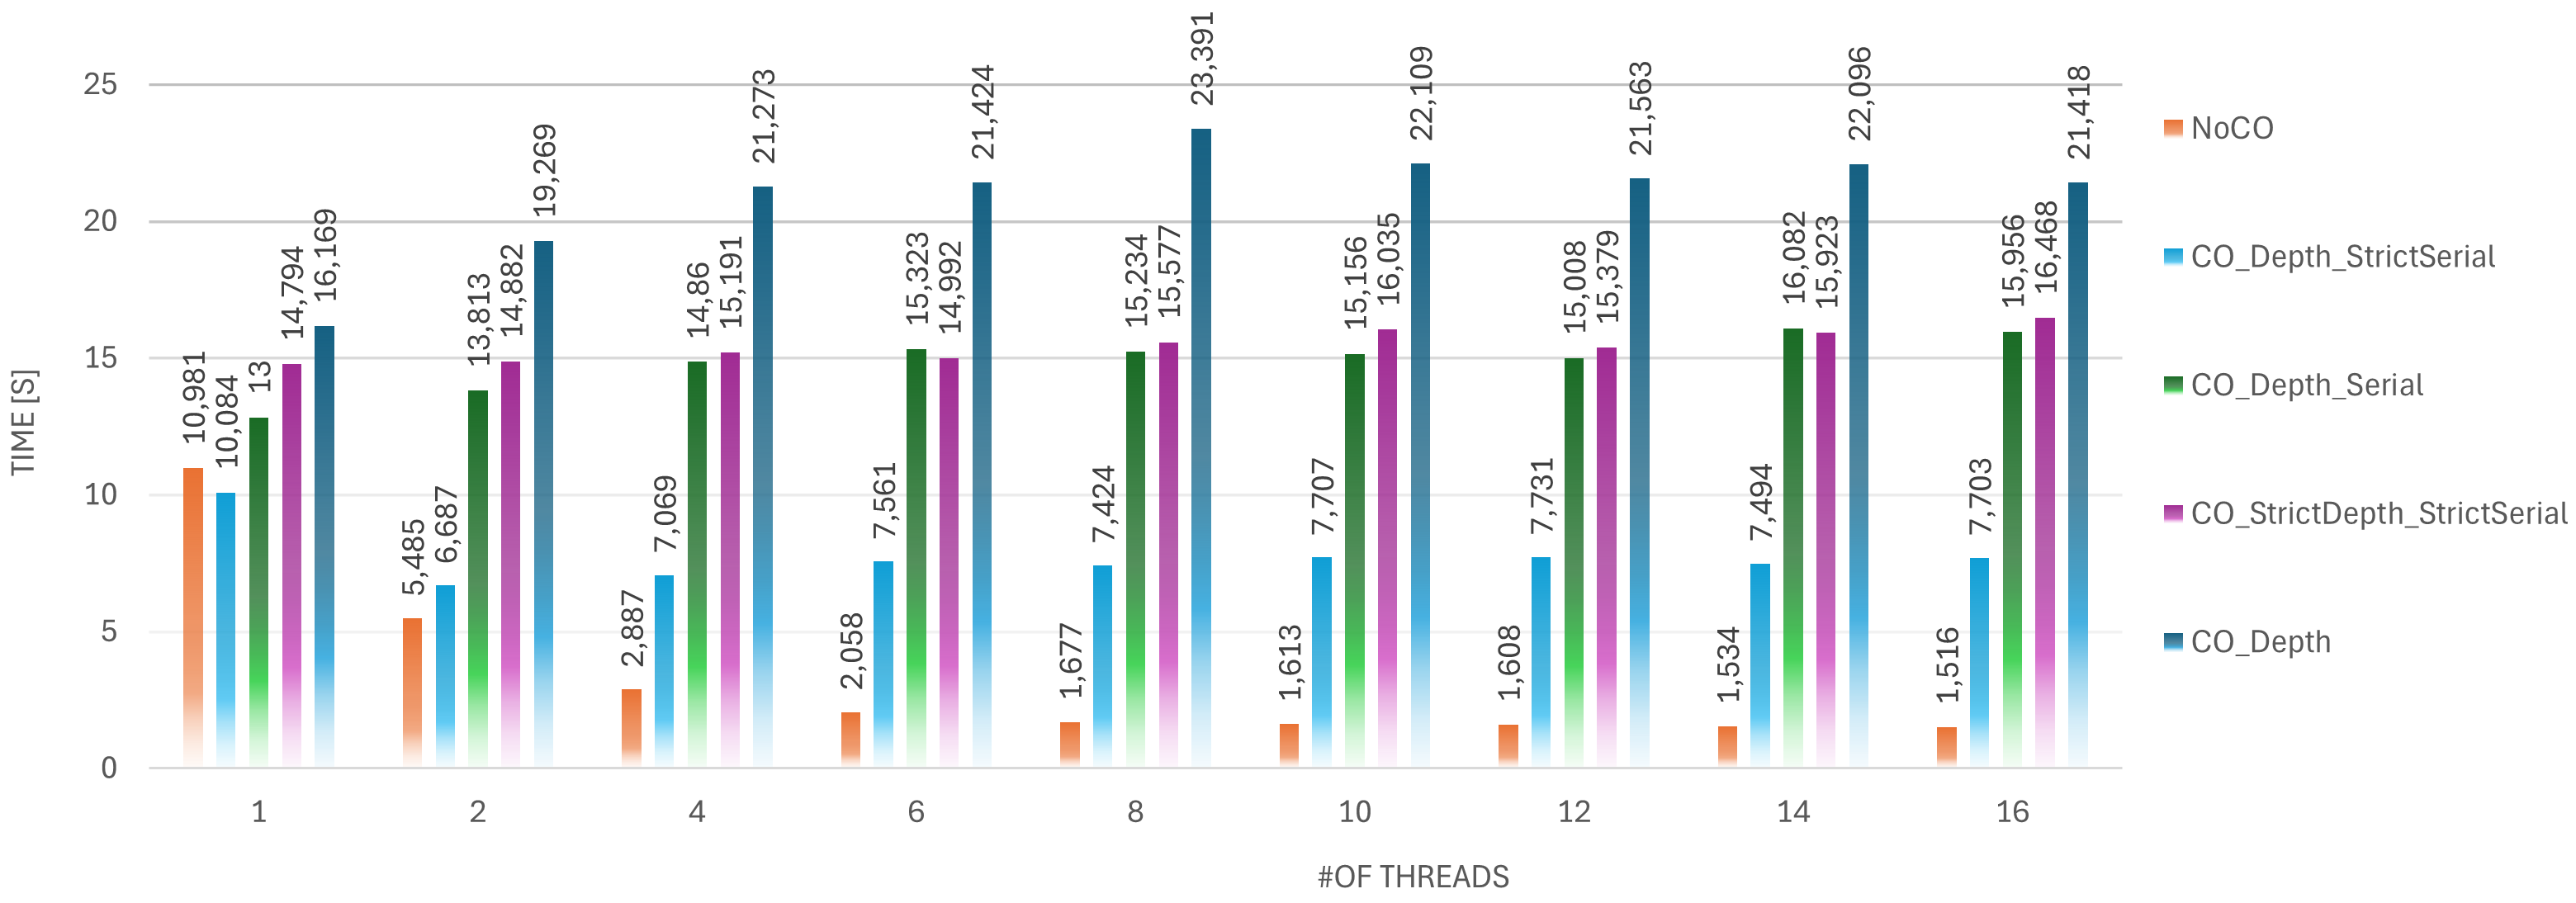
\includegraphics[width=1\linewidth]{image.png}
        \caption{Performance on a Intel Core i9-10850K}
    \end{figure}
    
    The performance of the algorithm varied significantly across different hardware setups.
    This variability demonstrates that parallel algorithms must be fine-tuned for the specific machine they are run on.

    \section{Design choices}
    The Sudoku solver was implemented using a brute-force approach based on Depth-First Search (DFS). 
    Each empty cell in the Sudoku grid is filled by recursively attempting all valid numbers, backtracking when a conflict is encountered.
    To optimize performance and manage the computational demands of the problem, we incorporated OpenMP to parallelize the recursive calls. 
    This was achieved by creating OpenMP tasks at each recursive level. 
    However, this approach faced two major challenges:
    \begin{enumerate}
        \item \textit{Excessive number of tasks:} for large Sudoku puzzles, the number of parallel tasks generated could grow exponentially, overwhelming system resources.
        \item \textit{High memory usage:} at each node of the recursion tree, a new Sudoku board had to be created and stored, leading to significant memory consumption.
    \end{enumerate}
    \noindent To address these challenges, we introduced cutoff strategies:
    \begin{itemize}
        \item \textit{Depth-based cutoff:} tasks are generated only at specific levels of recursion, i.e. $n$ levels. 
            This reduces the number of parallel tasks while maintaining the benefits of parallelism, to reduce overheads and memory.
        \item \textit{Serial algorithm cutoff:} tlast levels of recursion are solved using a serial implementation. 
            This approach significantly reduces memory usage as the serial algorithm modifies the Sudoku board in place, eliminating the need to copy the board at every step.
        \item \textit{Combination of cutoffs:} a combination of the depth-based and serial cutoffs was also implemented to test their combined effectiveness, in two configurations:
            \begin{itemize}
                \item \textit{Strict configuration:} the depth-based cutoff occurs more frequently, so the tasks are generated every larger $n$ level, and the serial cutoff is applied at a lower level. 
                    This reduces the number of tasks and memory usage more aggressively.
                    \item \textit{Non-strict configuration}.
            \end{itemize}
    \end{itemize}
    These design choices allowed us to systematically explore the trade-offs between parallelism, memory usage, and computational overhead. 
    The different cutoff configurations were evaluated to determine their impact on performance for various Sudoku inputs.
\end{document}